\documentclass[titlepage,letterpaper,dvips,landscape,20pt]{foils}

\usepackage{latexsym,verbatim,ams,amssymb}
\usepackage[dvips]{graphicx,color}

\definecolor{title}{rgb}{0,0,0.9}
\definecolor{titleback}{rgb}{0.87,1,0.82}
\definecolor{slidetitle}{rgb}{0,0,0.9}
\definecolor{slidetitlebg}{rgb}{0.8,1,0.8}
\definecolor{pseudocode}{rgb}{0.0,0.6,0.0}
\definecolor{emphisize}{rgb}{0.8,0,0}

\MyLogo{}

\Restriction{\textbf{25 A\~{N}OS DE LA COMPUTACI\'{O}N EN EL CINVESTAV}}

\setlength{\textheight}{6.28in}
\topmargin -40pt 

\newcommand{\bO}{\mbox{\cal O}}
\newcommand{\bA}{{\bf A}}
\newcommand{\bif}{{\bf if }}
\newcommand{\bff}{{\bf function }}
\newcommand{\bthen}{{\bf then }}
\newcommand{\belse}{{\bf else }}
\newcommand{\bfor}{{\bf for }}
\newcommand{\bdownto}{{\bf downto }}
\newcommand{\bto}{{\bf to }}
\newcommand{\bret}{{\bf return }}
\newcommand{\bbegin}{{\bf begin }}
\newcommand{\bend}{{\bf end }}
\newcommand{\bwhile}{{\bf while }}
\newcommand{\bdo}{{\bf do }}

\newcommand{\bit}{\begin{itemize}}
\newcommand{\eit}{\end{itemize}}
\newcommand{\ben}{\begin{enumerate}}
\newcommand{\een}{\end{enumerate}}
\newcommand{\bed}{\begin{description}}
\newcommand{\eed}{\end{description}}
\newcommand{\edo}{\end{document}}
\newcommand{\bce}{\begin{center}}
\newcommand{\ece}{\end{center}}

\begin{document}

\title{25 Years of Cryptographic Hardware Design \\[2cm]}

\author{\Large{\c{C}etin Kaya Ko\c{c}} \\[1em]
City University of Istanbul \& \\
University of California Santa Barbara \\[2em]
\texttt{koc@cs.ucsb.edu}\\
\texttt{http://cryptocode.net}\\
\texttt{koc@cryptocode.net}
}

\date{}

\maketitle

\foilhead[-0.5in] {\ \setlength\fboxrule{2pt}
\fcolorbox{slidetitle}{titleback} {\
\makebox[607pt]{\color{slidetitle}
25 Years of Cryptographic Hardware Design
}}}

\bit
\item 1975-1977: Invention of Public-Key Cryptography
\item Diffie-Hellman \& RSA Algorithms
\item Publication Dates: Nov 1976 \& Feb 1978
\item First hardware implementation: 

R. L. Rivest. A Description of a Single-Chip Implementation of the
RSA Cipher. \textsl{Lambda}, vol. 1, pages 14-18, 1980.
    
\item In 1984, I was a graduate student at UCSB's ECE Department
\item My interest started with Rivest's hardware paper

\eit

\foilhead[-0.5in] {\ \setlength\fboxrule{2pt}
\fcolorbox{slidetitle}{titleback} {\
\makebox[607pt]{\color{slidetitle}
Essential Milestones
}}}

\bit
\item This talk gives a brief summary of advanced algorithms 
for creating better hardware
realizations of public-key cryptographic algorithms: Diffie-Hellman, RSA,
elliptic curve cryptography
\item Essential milestones:
 \bit
 \item Naive algorithms, 1978-1985
 \item Montgomery algorithm, 1985
 \item Advanced Karatsuba algorithms, 1994
 \item Advanced Montgomery algorithms, 1996
 \item Montgomery algorithm in $GF(2^k)$, 1998
 \item Unified arithmetic, 2002
 \item Spectral arithmetic, 2006
 \eit

\eit

\foilhead[-0.5in] {\ \setlength\fboxrule{2pt}
\fcolorbox{slidetitle}{titleback} {\
\makebox[607pt]{\color{slidetitle}
RSA Computation
}}}

\bit
\item
The RSA algorithm uses modular exponentiation for encryption
\[
C := M^e \pmod{n}
\]
and decryption
\[
M : C^d \pmod{n}
\]
\item The computation of $M^e \bmod{n}$ is performed using
exponentiation heuristics

\item Modular exponentiation requires
implementation of three basic modular arithmetic operations:
addition, subtraction, and multiplication

\eit

\foilhead[-0.5in] {\ \setlength\fboxrule{2pt}
\fcolorbox{slidetitle}{titleback} {\
\makebox[607pt]{\color{slidetitle}
Diffie-Hellman Computation
}}}

\bit
\item Similarly, the Diffie-Hellman key exchange algorithm executes
the steps
\begin{eqnarray*}
R_A & := & g^a \pmod{p} \\
R_B & := & g^b \pmod{p} \\
R_{B}' & := & R_A^b = g^{ab} \pmod{p} \\
R_{A}' & := & R_B^a = g^{ba} \pmod{p}
\end{eqnarray*}
between two parties, Alice \& Bob
\item These computations are also modular exponentiations,
requiring modular addition, subtraction, and multiplication
operations

\eit

\foilhead[-0.5in] {\ \setlength\fboxrule{2pt}
\fcolorbox{slidetitle}{titleback} {\
\makebox[607pt]{\color{slidetitle}
NIST Digital Signature Algorithm
}}}

\bit
\item The signature computation on $M$ and $k$ is the pair $(r,s)$
\begin{eqnarray*}
r & := & (g^k \bmod{p}) \bmod{q} \\
s & := & (M+ x r)k^{-1} \bmod{q}
\end{eqnarray*}
\item The signature verification
\begin{eqnarray*}
w   & := & s^{-1} \bmod{q} \\
u_1 & := & M w    \bmod{q} \\
u_2 & := & r w    \bmod{q} \\
v   & := & (g^{u_1} y^{u_2} \bmod{p}) \bmod{q} \\
\mbox{Check if~~} r & = & v
\end{eqnarray*}
\eit

\foilhead[-0.5in] {\ \setlength\fboxrule{2pt}
\fcolorbox{slidetitle}{titleback} {\
\makebox[607pt]{\color{slidetitle}
Ellliptic Curve Cryptography
}}}

\bit
\item Elliptic curves defined over $GF(p)$ or $GF(2^k)$ are used
in cryptography

\item The arithmetic of $GF(p)$ is the usual mod $p$ arithmetic

\item The arithmetic of $GF(2^k)$ is similar to that of $GF(p)$,
however, there are some differences

\item Elliptic curves over $GF(2^k)$ are
more popular due to the space and time-efficient algorithms
for doing arithmetic in $GF(2^k)$

\item Elliptic curve cryptosystems based on discrete logarithms
seem to provide similar amount of
security to that of RSA, but with relatively shorter key sizes
\eit


\foilhead[-0.5in] {\ \setlength\fboxrule{2pt}
\fcolorbox{slidetitle}{titleback} {\
\makebox[607pt]{\color{slidetitle}
Computations of Cryptographic Functions
}}}

\bit
\item It is interesting to note that all public-key cryptographic
algorithms are based on number-theoretic and algebraic finite
structures, such as groups, rings, and fields
\item In fact, most of them need modular arithmetic, i.e.,
the arithmetic of integers in finite rings or fields
\item The challenge is however that the sizes of operands are
large, starting from about 160 bits up to 16,000 bits
\item Therefore, the algorithmic development of cryptographic hardware 
design is essentially based on (exact) computer arithmetic with very
large integers
\item Since exponentiations \& multiplications are most time/energy/space
consuming computations, we will only study those in our talk
\eit

\foilhead[-0.5in] {\ \setlength\fboxrule{2pt}
\fcolorbox{slidetitle}{titleback} {\
\makebox[607pt]{\color{slidetitle}
Computing Exponentiations
}}}

\bit
\item Given the integer $e$, the computation of $M^e$ or $eP$
is an exponentiation operation

\item The objective is to use as few multiplications (or elliptic curve
additions) as possible for a given integer $e$

\item This problem is related to {\it addition chains}

\item An addition chain yields an algorithm for computing $M^e$ or $eP$
given the integer $e$
\[
M^1 \rightarrow
M^2 \rightarrow
M^3 \rightarrow
M^5 \rightarrow
M^{10} \rightarrow
M^{11} \rightarrow
M^{22} \rightarrow
M^{44} \rightarrow
M^{55}
\]
\[
P \rightarrow
2P \rightarrow
3P \rightarrow
5P \rightarrow
10P \rightarrow
11P \rightarrow
22P \rightarrow
44P \rightarrow
55P
\]


\eit

\foilhead[-0.5in] {\ \setlength\fboxrule{2pt}
\fcolorbox{slidetitle}{titleback} {\
\makebox[607pt]{\color{slidetitle}
Computing Exponentiations
}}}

\bit
\item Finding the shortest addition chain is an NP-complete problem

\item Lower bound: $\log_2 e + \log_2 H(e) -2.13$
({\em Sch\"{o}nhage})

\item Upper bound: $\lfloor \log_2 e \rfloor  +H(e)-1$, where
$H(e)$ is the Hamming weight of $e$ 
(the binary method, the SX method, {\em Knuth})

\item It turns out the oldest known algorithm for computing
exponentiation is not too far in efficiency
to the best algorithm

\item Heuristics, $m$-ary, adaptive $m$-ary, sliding
windows, power tree methods offer only slight improvements

\eit


\foilhead[-0.5in] {\ \setlength\fboxrule{2pt}
\fcolorbox{slidetitle}{titleback} {\
\makebox[607pt]{\color{slidetitle}
Computing Modular Multiplication - Naive Algorithms
}}}

\bit
\item Given $a,b<n$, compute $P=a\cdot b \bmod{n}$
\item Multiply and reduce:

Multiply: $P' = a \cdot b$ ($2k$-bit number)

Reduce: $P = P' \bmod{n}$ ($k$-bit number)

\item Reductions are essentially integer divisions

\item However, multiply and reduce steps can be interleaved,
but offering only slight improvements

\eit

\foilhead[-0.5in] {\ \setlength\fboxrule{2pt}
\fcolorbox{slidetitle}{titleback} {\
\makebox[607pt]{\color{slidetitle}
Interleaved Multiply \& Reduce - Naive Algorithms
}}}

\begin{eqnarray*}
P' & = & a \cdot b = a \cdot \sum_{i=0}^{k-1}b_i2^i
                   = \sum_{i=0}^{k-1}(a \cdot b_i) 2^i \\[0.5em]
   & = &  2(\cdots 2(2(0+a\cdot b_{k-1})+
         a\cdot b_{k-2})+\cdots)+a\cdot b_0
\end{eqnarray*}

\begin{tabbing}
\=xxxxx\= \kill
\>1.     \> $P:=0$ \\
\>2.     \> \bfor \= $i=k-1$ \bdownto $0$\\
\>2a.    \>       \> $P := 2P + a \cdot b_i$ \\
\>2b.    \>       \> $P := P \bmod{n}$ \\
\>3.     \> \bret $P$
\end{tabbing}
\bit
\item Unfortunately, Step 2b is highly time consuming (a 
full division for every bit of the operands)
\eit

\foilhead[-0.5in] {\ \setlength\fboxrule{2pt}
\fcolorbox{slidetitle}{titleback} {\
\makebox[607pt]{\color{slidetitle}
Montgomery Multiplication - 1985
}}}

\bit
\item Attempts to create good hardware to compute the RSA functions
(sign, verify, encrypt, decrypt) in acceptable time have essentially 
failed because of the excessive requirements of the naive algorithms
\item This includes Rivest's hardware proposal and all other
implementations until the Montgomery multiplication algorithm
came about
\item Peter Montgomery discovered a method to replace Step 2b
with a step similar to Step 2a: an addition instead of a division
\item It is brilliant and efficient
\item Montgomery's algorithm changed cryptographic design 
in a way very much like the FFT algorithm changed the digital signal
processing
\eit


\foilhead[-0.5in] {\ \setlength\fboxrule{2pt}
\fcolorbox{slidetitle}{titleback} {\
\makebox[607pt]{\color{slidetitle}
Montgomery Multiplication
}}}

\bit
\item Montgomery's method maps the integers $\{0,1,2,\ldots,n-1\}$
to the same set with the map $\bar{x}= x \cdot r \pmod{n}$ using
the integer $r=2^k$
\item It then works in this set (numbers with the ``bar'' sign) and
performs the multiplication
\[
\mbox{MonPro}(\bar{a},\bar{b})=\bar{a} \cdot \bar{b} \cdot 2^{-k} \pmod{n}
\]
\item The above operation turns out to be significantly simpler than
the standard modular multiplication
$a \cdot b \pmod{n}$ because the division by $n$ in Step 2b (reduction)
is avoided
\item Transformation to and back from the ``bar'' domain is also
quite easily done, i.e., 
$\bar{x}=\mbox{MonPro}(x,r^2)$ and
$x=\mbox{MonPro}(\bar{x},1)$
 

\eit

\foilhead[-0.5in] {\ \setlength\fboxrule{2pt}
\fcolorbox{slidetitle}{titleback} {\
\makebox[607pt]{\color{slidetitle}
Montgomery Multiplication
}}}

\bit
\item In order to compute $u=\mbox{MonPro}(a,b)=a \cdot b \cdot 2^{-k}
\pmod{n}$, we use the steps below
\begin{tabbing}
\=1. \quad \= $u:=0$ \\
\>2.       \> \textbf{for} \= $i=0$ \textbf{to} $k-1$ \\
\>2a.      \> \> $u:=u+a_i \cdot b$ \\
\>2b.      \> \> \textbf{if} $u_0$ is 1 \textbf{then} $u:=u+n$ \\
\>3.       \> \> $u:=u/2$
\end{tabbing}
\item Now, Step 2b is only an addition! 
\item And, it is is done about half of the time!
\item We remain in the Montgomery (``bar'') domain of integers until
the final step of the exponentiation, and then use the
conversion routine to go back to the ``no bar'' domain
\eit

\foilhead[-0.5in] {\ \setlength\fboxrule{2pt}
\fcolorbox{slidetitle}{titleback} {\
\makebox[607pt]{\color{slidetitle}
Karatsuba-Ofman Multiplication
}}}

\bit
\item Algorithms Textbooks offer a few asymptotically faster multiplication
algorithms: Karatsuba-Ofman, Toom-Cook, Winograd, and DFT-based algorithms
\item These algorithms are all good: they help you to multiply faster
\item But, they are no help in modular multiplication, i.e., they do not
multiply-and-reduce (Montgomery's method is special)
\item They also have large overhead, and start being faster only after
a few thousand bits
\item However, there has been significant algorithmic developments
to bring down their break-even point to a few hundred bits

\eit

\foilhead[-0.5in] {\ \setlength\fboxrule{2pt}
\fcolorbox{slidetitle}{titleback} {\
\makebox[607pt]{\color{slidetitle}
Advanced Montgomery Multiplication
}}}

\bit
\item On the other hand, Montgomery algorithms also improved
\item They can be made fit into specific archiectures, by changing
the way they scan the bits of the multiplicand, the multiplier, 
and the product
\item Separated Operand Scanning (SOS):
First computes $t= a \cdot b$ and then interleaves
the computations of $m=t \cdot n' \bmod{r}$ and
$u=(t+ m \cdot n)/r$. Squaring can be optimized.

SOS requires $2s+2$ words of space

\item Finely Integrated Product Scanning (FIPS):
Interleaves computation of $a \cdot b$ and $m \cdot n$
by scanning the words of $m$

It uses the same space to keep $m$ and $u$,
reducing the temporary space to $s+3$ words

\eit

\foilhead[-0.5in] {\ \setlength\fboxrule{2pt}
\fcolorbox{slidetitle}{titleback} {\
\makebox[607pt]{\color{slidetitle}
Advanced Montgomery Multiplication
}}}

\bit
\item Finely Integrated Operand Scanning (FIOS):
The computation of $a \cdot b$ and $m \cdot n$ is performed
in a single loop

FIOS also requires $s+3$ words of space

\item Coarsely Integrated Hybrid Scanning (CIHS):
The computation of $a \cdot b$ is split into 2 loops, and
the second loop is interleaved with the computation of
$m\cdot n$

CIHS also requires $s+3$ words of space

\item Coarsely Integrated Operand Scanning(CIOS):
Improves the SOS method by integrating the multiplication and
reduction steps. It alternates between iterations
of the outer loops for multiplication and reduction

CIOS also requires $s+3$ words of space

\eit

\foilhead[-0.5in] {\ \setlength\fboxrule{2pt}
\fcolorbox{slidetitle}{titleback} {\
\makebox[607pt]{\color{slidetitle}
Advanced Montgomery Multiplication
}}}

\bit
\item All methods require $2s^2+s$ multiplications
\item Add, Read/Write and Space requirements are below
\eit

\begin{center}
\begin{tabular}{|l|l|l|l|r|} \hline
 & {\small Add} & {\small Read/Write} & {\small Space} \\ \hline
{\small SOS}  & ${\scriptstyle 4s^2+4s+2}$
              & ${\scriptstyle 8s^2+13s+5}$
              & ${\scriptstyle 2s+2}$ \\
{\small FIPS} & ${\scriptstyle 6s^2+2s+2}$
              & ${\scriptstyle 14s^2+16s+3}$
              & ${\scriptstyle s+3}$ \\
{\small FIOS} & ${\scriptstyle 5s^2+3s+2}$
              & ${\scriptstyle 10s^2+9s+3}$
              & ${\scriptstyle s+3}$ \\
{\small CIHS} & ${\scriptstyle 4s^2+4s+2}$
              & ${\scriptstyle 9.5s^2+11.5s+3}$
              & ${\scriptstyle s+3}$ \\
{\small CIOS} & ${\scriptstyle 4s^2+4s+2}$
              & ${\scriptstyle 8s^2+12s+3}$
              & ${\scriptstyle s+3}$ \\ \hline
\end{tabular}
\end{center}

\bit
\item Depending on the availability of functional units
(multipliers, adders, registers), one method can outperform
another and thus should be selected
\eit

\foilhead[-0.5in] {\ \setlength\fboxrule{2pt}
\fcolorbox{slidetitle}{titleback} {\
\makebox[607pt]{\color{slidetitle}
Montgomery Multiplication in $GF(2^k)$
}}}

\bit
\item It turns out that the Montgomery multiplication can also
be performed in the finite field $GF(2^k)$ if the polynomial
basis representations of the field elements are employed
\item It imitates the the Montgomery multiplication in $GF(p)$
by taking the modulus the irreducible polynomial $p(x)$ generating
the field of $2^k$ elements
\item It is not as fast as the normal basis, but it has some advantages
\eit

\foilhead[-0.5in] {\ \setlength\fboxrule{2pt}
\fcolorbox{slidetitle}{titleback} {\
\makebox[607pt]{\color{slidetitle}
Montgomery Multiplication in $GF(2^k)$
}}}

\bit
\item In order to compute 
\[
u(x)=\mbox{MonPro}(a(x),b(x))=a(x) \cdot b(x) \cdot x^{-k} \bmod{p(x)}~,
\] 
we use the steps below

\begin{tabbing}
\=1. \quad \= $u(x):=0$ \\
\>2.       \> \textbf{for} \= $i=0$ \textbf{to} $k-1$ \\
\>2a.      \> \> $u(x):=u(x)+a_i \cdot b(x) \bmod{2}$ \\
\>2b.      \> \> \textbf{if} $u_0$ is 1 \textbf{then} $u(x) := u(x)+p(x) \bmod{2}$ \\
\>3.       \> \> $u:=u/2$
\end{tabbing}

\item Now Steps 2a and 2b use mod 2 additions (XOR gates) 
\eit

\foilhead[-0.5in] {\ \setlength\fboxrule{2pt}
\fcolorbox{slidetitle}{titleback} {\
\makebox[607pt]{\color{slidetitle}
Unified Arithmetic
}}}

\bit
\item One advantage of the Montgomery multiplication in $GF(2^k)$ is that
a single arithmetic unit can be used to handle both kinds of fields: $GF(p)$
and $GF(2^k)$: This is called unified arithmetic (or, dual-field arithmetic)
\item Advantages of the unified arithmetic are low manufacturing cost,
compatibility, parallelism, and \textsl{scalability} 
\item Furthermore, unified arithmetic is impartial: it does not favor
one prime against another or one irreducible polynomial against another
\item The building block of the unified architecture is the
unified full adder: a 1-bit adder that handles both $GF(p)$ and
$GF(2^k)$

\eit

\foilhead[-0.5in] {\ \setlength\fboxrule{2pt}
\fcolorbox{slidetitle}{titleback} {\
\makebox[607pt]{\color{slidetitle}
Unified Full Adder
}}}

\vspace*{2cm}

\begin{center}
\includegraphics[width=20cm]{ufa.eps}
\end{center}

\foilhead[-0.5in] {\ \setlength\fboxrule{2pt}
\fcolorbox{slidetitle}{titleback} {\
\makebox[607pt]{\color{slidetitle}
Scalability
}}}

\bit

\item \textsl{Scalability} is an important concept: it allows
to make small changes in the hardware to handle larger operands
without a complete redesign (such as switching from 1024-bit RSA
keys to 1536-bit RSA keys)

\eit

\begin{center}
\includegraphics[width=20cm]{scale.eps}
\end{center}

\foilhead[-0.5in] {\ \setlength\fboxrule{2pt}
\fcolorbox{slidetitle}{titleback} {\
\makebox[607pt]{\color{slidetitle}
Dependency Graph of Montgomery Multiplication
}}}

\begin{center}
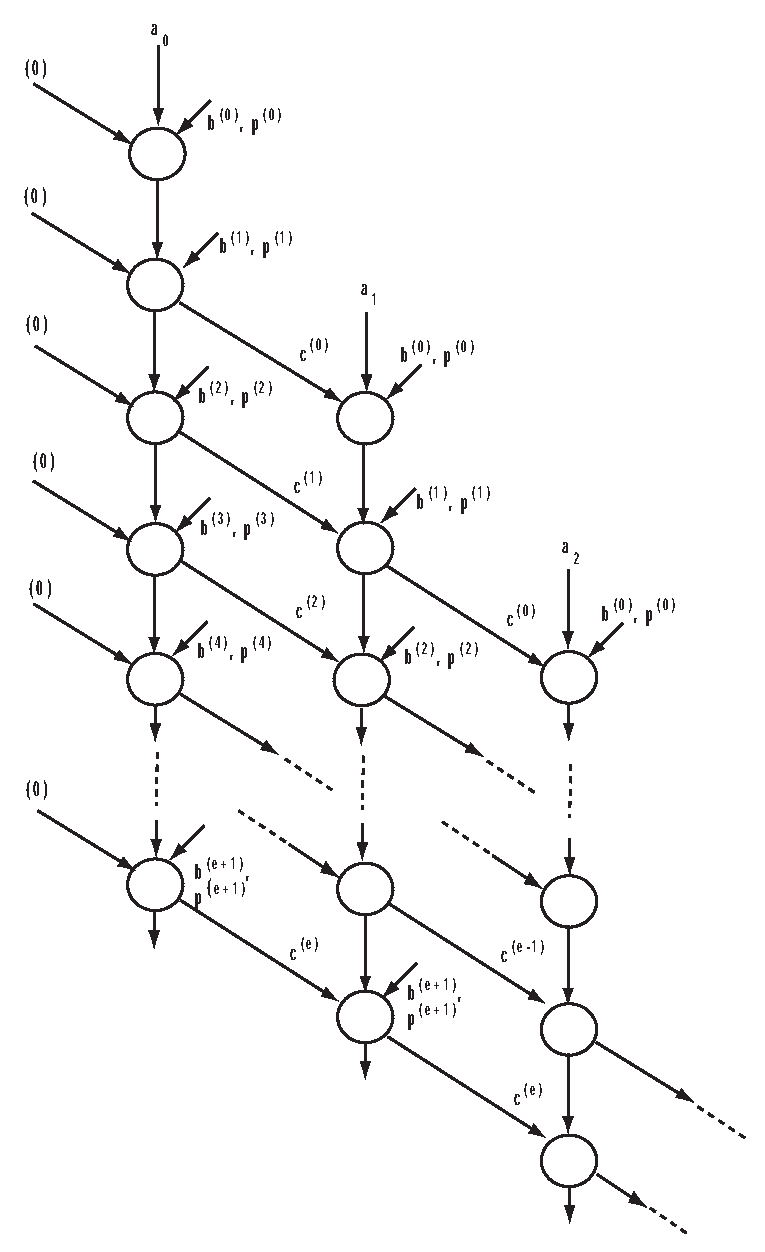
\includegraphics[width=8cm]{dependency.eps}
\end{center}

\foilhead[-0.5in] {\ \setlength\fboxrule{2pt}
\fcolorbox{slidetitle}{titleback} {\
\makebox[607pt]{\color{slidetitle}
Pipelined Montgomery Multiplication
}}}

\begin{center}
\includegraphics[width=20cm]{pipeline1.eps}
\end{center}

\foilhead[-0.5in] {\ \setlength\fboxrule{2pt}
\fcolorbox{slidetitle}{titleback} {\
\makebox[607pt]{\color{slidetitle}
Pipelined Architecture with Fewer Units
}}}

\begin{center}
\includegraphics[width=20cm]{pipeline2.eps}
\end{center}

\foilhead[-0.5in] {\ \setlength\fboxrule{2pt}
\fcolorbox{slidetitle}{titleback} {\
\makebox[607pt]{\color{slidetitle}
General Pipelined Architecture
}}}

\begin{center}
\includegraphics[width=20cm]{pipeline3.eps}
\end{center}

\foilhead[-0.5in] {\ \setlength\fboxrule{2pt}
\fcolorbox{slidetitle}{titleback} {\
\makebox[607pt]{\color{slidetitle}
Spectral Arithmetic
}}}

\bit
\item We use FFT-based arithmetic to implement 
\textsl{modular multiplication}

\item However, we are interested in performing the reduction inside
the spectral (frequency) domain

\item We utilize finite ring and field arithmetic (avoid real or
complex arithmetic because of the roundoff errors in using
floating-point or fixed-point arithmetic)

\item We also want to bring down the break-even point of efficiency
for FFT-based multiplication

\item Furthermore, we utilize the properties of the
DFT and Montgomery algorithm to perform \textsl{modular multiplication}


\eit

\foilhead[-0.5in] {\ \setlength\fboxrule{2pt}
\fcolorbox{slidetitle}{titleback} {\
\makebox[607pt]{\color{slidetitle}
Spectral Arithmetic
}}}

\vspace*{2cm}

\begin{center}
\includegraphics{fig3.eps}
\end{center}

\foilhead[-0.5in] {\ \setlength\fboxrule{2pt}
\fcolorbox{slidetitle}{titleback} {\
\makebox[607pt]{\color{slidetitle}
DFT over a Finite Ring: Definition
}}}

\noindent Let $\omega$ be a primitive $d$-th root of unity in
$\mathbb{Z}_q$ and, let $x(t)$ and $X(t)$ be polynomials of degree $d-1$
having entries in $\mathbb{Z}_q$. The DFT map over $\mathbb{Z}_q$ is an invertib
le
set map sending  $x(t)$ to $X(t)$ given by
\[
X_i = DFT_d^{\omega}(x(t)) := \sum_{j=0}^{d-1} x_j\omega^{i j} \bmod q,
\]
with the inverse
\[ 
x_i = IDFT_d^{\omega}(X(t)) := d^{-1} \cdot \sum_{j=0}^{d-1}
   X_j\omega^{-i j} \bmod q,
\]
for $i,j=0,1,\ldots,d-1$. 

\foilhead[-0.5in] {\ \setlength\fboxrule{2pt}
\fcolorbox{slidetitle}{titleback} {\
\makebox[607pt]{\color{slidetitle}
DFT over a Finite Ring: Existence
}}}

\noindent We write
\[
x(t) ~~ \begin{array}{c} \mbox{\tiny DFT} \\
                         \longleftrightarrow
        \end{array} ~~ X(t)
\]
and say $x(t)$ and $X(t)$ are transform pairs; $x(t)$ is called a
{\bf time polynomial} and sometimes $X(t)$ is named as the
{\bf spectrum} of $x(t)$.

\bit
\item (Convention)  In the literature, DFT over a finite ring spectrum
is also called as Number Theoretical Transform (NTT)
\item (Existence) In order to have a DFT map over ${\mathbb Z}_q$:
 \bit
 \item The multiplicative inverse of DFT length $d$  must exist in
 ${\mathbb Z}_q$ which requires that gcd$(d,q)=1$.
 \item $d$ has to divide $p-1$ for every prime $p$ divisor of $q$
 \eit
\eit

\foilhead[-0.5in] {\ \setlength\fboxrule{2pt}
\fcolorbox{slidetitle}{titleback} {\
\makebox[607pt]{\color{slidetitle}
DFT over a Finite Ring: Efficiency
}}}

\noindent In order to have simple arithmetic
\bit
\item $q$ should be chosen as \\
a Mersenne number $q = 2^v-1$, or \\
a Fermat number $q = 2^v+1$ 
\item The principal root of unity $\omega$ should
be selected as a power of 2 to simplify
the multiplications with roots of unity
\eit

\foilhead[-0.5in] {\ \setlength\fboxrule{2pt}
\fcolorbox{slidetitle}{titleback} {\
\makebox[607pt]{\color{slidetitle}
Properties of DFT
}}}

\bit
\item Under certain conditions, the Fourier transform preserves
some properties of the time sequences, e.g., linearity and convolution.
\item The existence conditions of these properties differ when working
in finite ring spectrums
\item Let $\phi$ and $\Phi$ be operations on time and spectral
domains respectively. We write
\[
\phi ~~ \begin{array}{c} \mbox{\tiny DFT} \\
                         \longleftrightarrow
         \end{array} ~~ \Phi
\]
and say $\phi$ and $\Phi$ are transform pairs on $x(t)$ and sometimes declare
that {\bf the map $DFT_d^{\omega}$ respects the operation $\phi$} on point
$x(t)$ if following equation is satisfied
\[
\phi(x(t)) = IDFT_d^{\omega} \circ \Phi \circ DFT_d^{\omega}(x(t))
\]
\eit

\foilhead[-0.5in] {\ \setlength\fboxrule{2pt}
\fcolorbox{slidetitle}{titleback} {\
\makebox[607pt]{\color{slidetitle}
Time-Frequency Dictionary
}}}

\bit
\item {\bf Time and frequency shifts}
correspond to circular shifts
Let \[
x(t)=x_0 + x_1 t + \ldots + x_{d-1}t^{d-1}
\]
and
\[
X(t)=X_0 + X_1t + \ldots + X_{d-1}t^{d-1}
\]
be a transform pair.

The {\em one-term right circular shift} is defined as $x(t) \circlearrowleft 1$
\[
\begin{array}{c}
x_{1} + x_2t + \ldots + x_{d-2}t^{d-1}+ x_{0}t^{d-1} \\
~~~~ \updownarrow  \mbox{\tiny DFT} \\
X(t) \odot \Gamma(t)
\end{array}
\]
where $\odot$ stands for component-wise multiplication and
\[
\Gamma(t) = 1 + \omega^{-1}t + \ldots + \omega^{-(d-1)}t^{d-1}
\]
\eit

\foilhead[-0.5in] {\ \setlength\fboxrule{2pt}
\fcolorbox{slidetitle}{titleback} {\
\makebox[607pt]{\color{slidetitle}
Time-Frequency Dictionary
}}}

\bit
\item {\bf Sum of sequence and first value:} The sum of the coefficients
of a time polynomial equals to the zeroth coefficient
of its spectral polynomial.
Conversely the sum of the spectrum coefficients equals
to $d^{-1}$ times the zeroth coefficient of the time polynomial

\[
x_0 = d^{-1} \cdot \sum_{i=0}^{d-1} X_i\omega^{-i}
~~~\mbox{and}~~~
X_0 = \sum_{i=0}^{d-1} x_i\omega^{i}
\]
\eit
\begin{center}
\includegraphics[height=2in]{fig7.eps}
\end{center}

\foilhead[-0.5in] {\ \setlength\fboxrule{2pt}
\fcolorbox{slidetitle}{titleback} {\
\makebox[607pt]{\color{slidetitle}
Time-Frequency Dictionary
}}}

\bit
\item {\bf Left and right logical shifts:} By using the previous  properties,
it is possible to perform logical left and right digit shifts $x(t) \ll 1$
as follows:
\[
\begin{array}{c}
(x(t)-x_0)/t = x_1 + \ldots + x_{d-1}t^{d-2} \\
~~~~~~~~~~~~~~~~ \updownarrow  \mbox{\tiny DFT} \\
(X(t) - x_0(t)) \odot \Gamma(t)
\end{array}
\]
where
\[
x_0(t) = x_0 + x_0t+x_0t^2+\ldots+x_0t^{d-1}
\]
\item The right shifts are similar, where one then uses the
\[
\Omega(t) = 1 + \omega^{1}t + \ldots + \omega^{(d-1)}t^{d-1}
\]
polynomial instead of $\Gamma(t)$
\eit

\foilhead[-0.5in] {\ \setlength\fboxrule{2pt}
\fcolorbox{slidetitle}{titleback} {\
\makebox[607pt]{\color{slidetitle}
A Time Simulation for Spectral Modular Multiplication
}}}

\noindent We would like to compute $859^2 \cdot 4^{-9}  \pmod{1337}$.\\
Signal $x(t)$ representing $859=x(4)$ in base 4.

\vspace*{0.5cm}
\bce
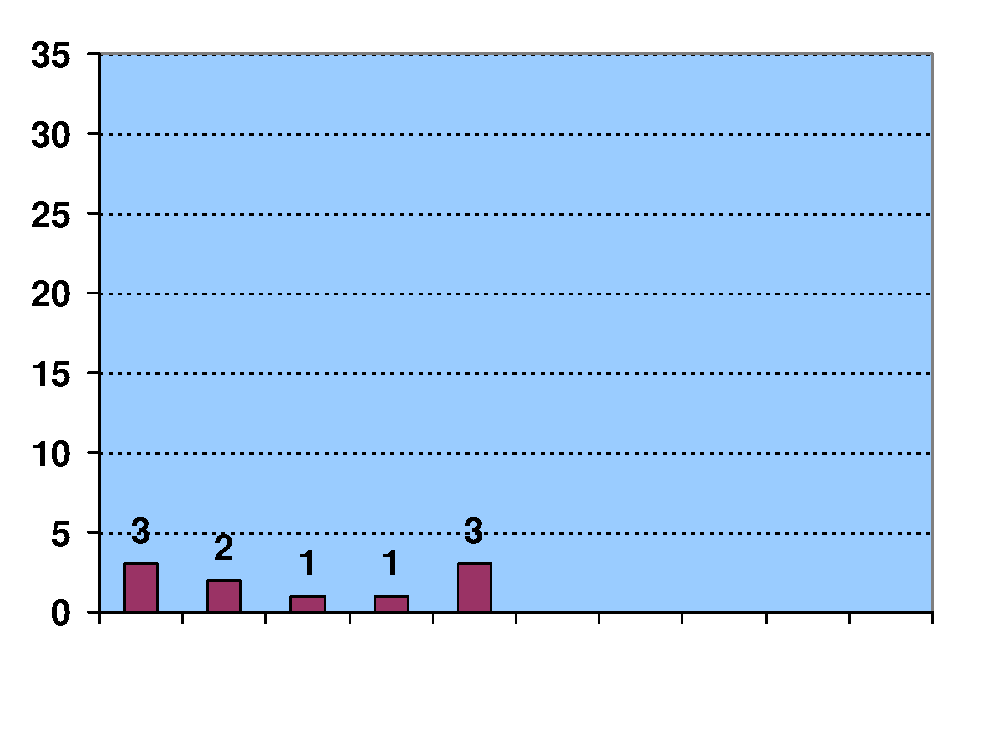
\includegraphics[width=5in]{fig8.eps}
\ece

\foilhead[-0.5in] {\ \setlength\fboxrule{2pt}
\fcolorbox{slidetitle}{titleback} {\
\makebox[607pt]{\color{slidetitle}
A Time Simulation for SMP
}}}

\noindent Convolving $x(t)$ with itself, we find
$x^2(t) = 859^2=737881$.

\vspace{0.5cm}
\bce
\includegraphics[width=5in]{fig9.eps}
\ece

\foilhead[-0.5in] {\ \setlength\fboxrule{2pt}
\fcolorbox{slidetitle}{titleback} {\
\makebox[607pt]{\color{slidetitle}
A Time Simulation for SMP
}}}

\noindent The modulus $m=1337$ is represented as $m=1+2t+3t^2+t^4+t^5$.We add $3m$ to the sum to anhilate the least significant $b$ bits of the least digit.

\vspace{0.5cm}
\bce
\includegraphics[width=5in]{figa.eps}
\ece

\foilhead[-0.5in] {\ \setlength\fboxrule{2pt}
\fcolorbox{slidetitle}{titleback} {\
\makebox[607pt]{\color{slidetitle}
A Time Simulation for SMP
}}}

\noindent Carry goes to the next digit.

\vspace{0.5cm}
\bce
\includegraphics[width=5in]{figb.eps}
\ece

\foilhead[-0.5in] {\ \setlength\fboxrule{2pt}
\fcolorbox{slidetitle}{titleback} {\
\makebox[607pt]{\color{slidetitle}
A Time Simulation for SMP
}}}

\noindent We then shift the digits.

\vspace{0.5cm}
\bce
\includegraphics[width=5in]{figc.eps}
\ece

\foilhead[-0.5in] {\ \setlength\fboxrule{2pt}
\fcolorbox{slidetitle}{titleback} {\
\makebox[607pt]{\color{slidetitle}
A Time Simulation for SMP
}}}

\noindent After 9 iterations, we find the result:
$914 \equiv 859^2 \cdot 4^{-9}  \pmod{1337}$.

\vspace{0.5cm}
\bce
\includegraphics[width=5in]{figd.eps}
\ece

\foilhead[-0.5in] {\ \setlength\fboxrule{2pt}
\fcolorbox{slidetitle}{titleback} {\
\makebox[607pt]{\color{slidetitle}
Unending Quest for Efficiency
}}}

\bit
\item Conclusions?
\item Challenges remain: Make faster but low-area and low-energy
hardware for cryptography
\item Platforms are diverse: Huge SSL and IPSec boxes versus 
tiny Bluetooth earphones, cellphones and PDAs
\item New challenges: We need to build countermeasures in order
to circumvent attacks by adversaries to obtain hardware-hidden secrets
\item Questions?

Email: koc@cryptocode.net

\eit 

\end{document}

